\section{Auswertung}
\label{sec:Auswertung}



\begin{table}
  \centering
  \caption{Eine Beispieltabelle mit Messdaten.}
  \label{tab:tabelle}
  \sisetup{table-format=1.1, per-mode=reciprocal}
  \begin{tblr}{
      colspec = {S[table-format=2.1] S[table-format=1.2] S},
      row{1} = {guard, mode=math},
      vline{4} = {2}{-}{text=\clap{$\pm$}},
    }
    \toprule
    x \mathbin{/} \unit{\volt} & I \mathbin{/} \unit{\milli\second} & \SetCell[c=2]{c} N \mathbin{/} \unit{\nano\ampere} & \\
    \midrule
   0.0 &   0.32   \\
   1.0 &   0.32   \\
   2.0 &   0.32   \\
   3.0 &   0.32   \\
   4.0 &   0.32   \\
   5.0 &   0.34   \\
   6.0 &   0.40   \\
   7.0 &   0.52   \\
   8.0 &   0.66   \\
   9.0 &   0.82   \\
  10.0 &   1.00   \\
  11.0 &   1.20   \\
  12.0 &   1.20   \\
  13.0 &   1.40   \\
  14.0 &   1.40   \\
  15.0 &   1.40   \\
  16.0 &   1.40   \\
  17.0 &   1.60   \\
  18.0 &   1.80   \\
  19.0 &   2.20   \\
  20.0 &   2.80   \\
  20.5 &   3.20   \\
  21.0 &   3.40   \\
  21.5 &   3.80   \\
  22.0 &   4.00   \\
  22.5 &   4.00   \\
  23.0 &   4.20   \\
  23.5 &   4.20   \\
  24.0 &   4.20   \\
  24.5 &   4.00   \\
  25.0 &   3.80   \\
  25.5 &   3.60   \\
  26.0 &   3.20   \\
  26.5 &   3.00   \\
  27.0 &   2.80   \\
  27.5 &   2.40   \\
  28.0 &   2.00   \\
  28.5 &   2.00   \\
  29.0 &   1.80   \\
  29.5 &   1.60   \\
  30.0 &   1.40   \\
  31.0 &   1.20   \\
  32.0 &   1.20   \\
  33.0 &   1.40   \\
  34.0 &   1.40   \\
  35.0 &   1.60   \\
  36.0 &   1.60   \\
  37.0 &   1.60   \\
  38.0 &   1.40   \\
  39.0 &   1.40   \\
  40.0 &   1.20   \\
  41.0 &   1.00   \\
  42.0 &   1.00   \\
  43.0 &   0.74   \\
  44.0 &   0.68   \\
  45.0 &   0.66   \\
  46.0 &   0.70   \\
  47.0 &   0.76   \\
  48.0 &   0.82   \\
  49.0 &   0.86   \\
  50.0 &   0.86   \\
    \bottomrule
  \end{tblr}
\end{table}

\begin{figure}
  \centering
  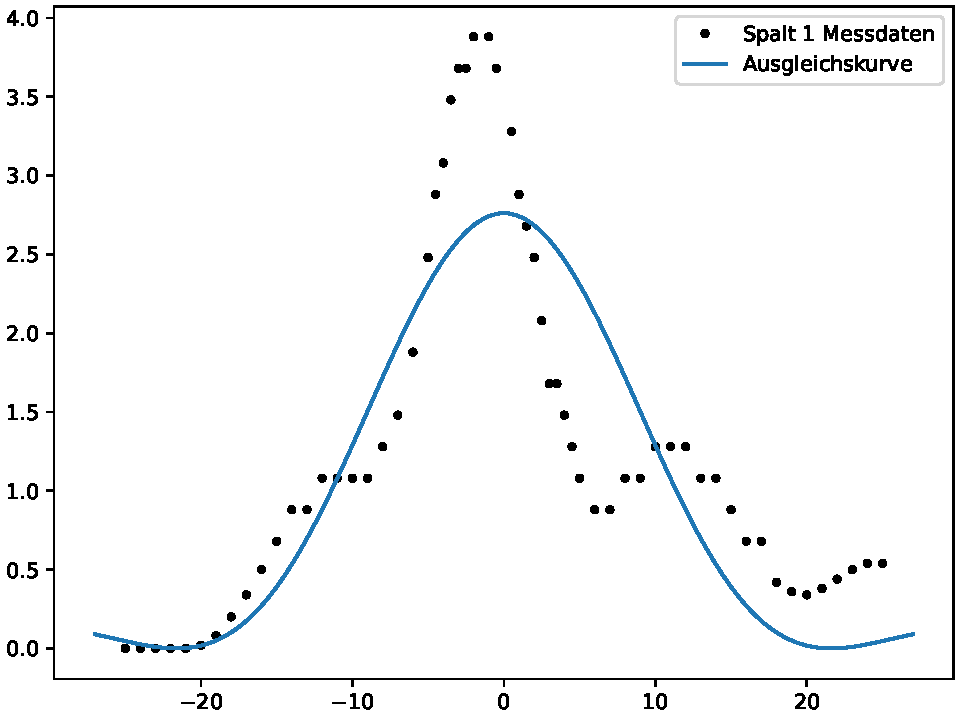
\includegraphics{plot.pdf}
  \caption{Plot.}
  \label{fig:plot}
\end{figure}

\begin{figure}
  \centering
  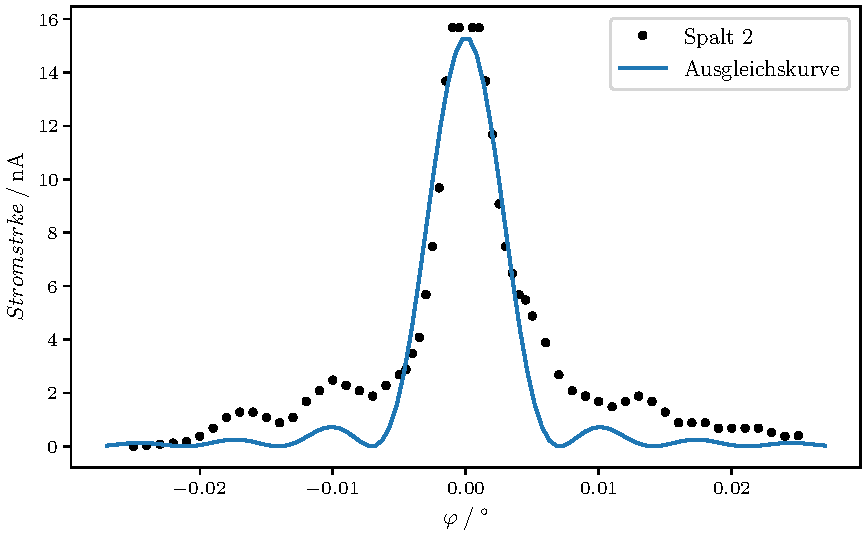
\includegraphics{plot1.pdf}
  \caption{Plot.}
  \label{fig:plot}
\end{figure}

\begin{figure}
  \centering
  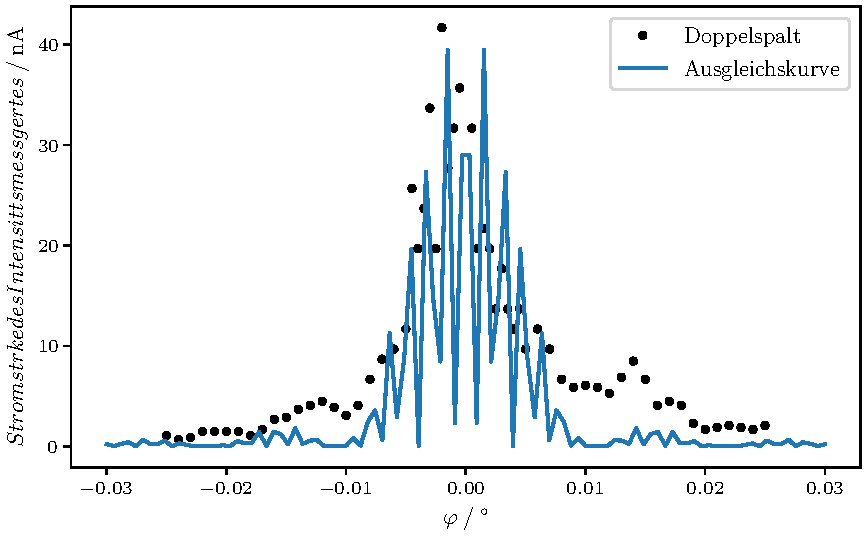
\includegraphics{plot2.pdf}
  \caption{Plot.}
  \label{fig:plot}
\end{figure}

